Apart from the applied density fitting method, the chosen orbital-free basis set arguably has an even greater impact on the accuracy of the density-fitted density. The commonly used even-tempered basis sets are reliable but often inefficient for defining an orbital-free basis. Their simple construction algorithm \cite{const} broadly covers the possible density space without refinement.

To improve the performance of our orbital-free basis set, it is sensible to adopt a basis set with higher resolution in regions where density fluctuates more rapidly. We construct this improved basis by beginning with an even-tempered set and using differentiable integrals and autograd.

\section{Using differentiable integrals to optimize an orbital free basis set}
Given differentiable basis integrals, we can describe the complete density fitting procedere in a completely differentiable way. For a given target density we want to optimize the L2 norm of the fitted density, so we are going to start with the overlap formulation of density ftting defined in \eqref{overlap_eq}. Other formulations using the residual hartree energy can also be easily formulated but they these integrals are much more costly to compute. We also found this formulation to be sufficient to optimize the relevant metrics to an acceptable level.
\begin{align}
    \mathcal{L}[\rho] &= \min_{\rho'}\left(||\rho-\rho'||_{\text{L2}}\right)\\
    & = \min_{\{p_{\mu}\}_{\mu \in 1,...,n_b}} \mathbf{p}W \mathbf{p} - 2 \mathbf{p} \bar L \bar\Gamma + \bar\Gamma \bar D \bar\Gamma\\
    & = \left[\mathbf{p} W \mathbf{p} - 2 \mathbf{p} \bar L \bar\Gamma+ \bar\Gamma \bar D \bar\Gamma\right]_{\mathbf{p} = W^{-1}\bar{L}\bar\Gamma}\\
    & = \bar \Gamma \bar L ^T W^{-1} \bar L \bar \Gamma - 2 \bar \Gamma \bar L^T W^{-1} \bar L \bar \Gamma + \bar \Gamma \bar D \bar \Gamma\\
    & = - \bar \Gamma \bar L^T W^{-1} \bar L \bar \Gamma + \bar \Gamma \bar D \bar \Gamma
\end{align}
We can now insert the dependency of our integrals on the exponents $\{\mathbf{\alpha}_Z\}_{Z\in \text{H,C,N,O,F}}$ for the gaussian basis functions for each atom.
The dependent integrals are the two center integral $W_{\mu,\nu}(\mathbf{\alpha}) = \langle \omega_\mu(\mathbf{\alpha})|\omega_\nu(\mathbf{\alpha})\rangle$
 and the three center overlap integral $L_{\mu,\gamma\sigma}(\mathbf{\alpha}) = \langle \omega_\mu(\mathbf{\alpha})|\eta_\gamma\eta_\sigma\rangle$. The 4 center overlap integral $D$ does not depend on the orbital free basis functions $\omega_\mu(\mathbf{\alpha})$ and can therefor be omitted from the final loss. For a single molecule geometry $\mathcal{M}$ we can define now our loss as
 \begin{align}\label{loss_basis_set_fitting}
    \text{Loss}_\text{molecule}(\mathcal{M}, \Gamma,\mathbf{\alpha}) & = - \bar \Gamma \bar L_{\mathcal{M}}^T(\mathbf{\alpha}) W_{\mathcal{M}}^{-1}(\mathbf{\alpha}) \bar L_{\mathcal{M}}(\mathbf{\alpha}) \bar \Gamma
 \end{align}
The loss of our entire dataset $\{\mathcal{M}_i,\Gamma_i\}_{i\in 1,...,N_{\text{molecules}}}$, containing the atomic structures and ground state densities, amounts to:
\begin{align} \label{loss_dataset_basis_set_fitting}
    \text{Loss}(\{\mathcal{M}_i,\Gamma_i\}_{i\in 1,...,N_{\text{molecules}}},\mathbf{\alpha}) = \sum\limits_{i=1}^{N_{\text{molecules}}} \text{Loss}_\text{molecule}(\mathcal{M}_i, \Gamma_i,\mathbf{\alpha})
\end{align}
For the atomic structures we used the molecules contained in the popular dataset QM9\ref{QM9}. For the target density we are using again the ground state density of a molecule generated by a kohn sham calculation using the PBE exchange correlation functional and the "6-31G(2df,p)" basis set for the orbitals.
As our entire framework is written in pytorch and differentiable the gradients of the loss of the single molecules can be computed by using pytorchs autograd. We can now minimize our loss function \eqref{loss_dataset_basis_set_fitting} by using stochastic gradient decent.\\
To shortly summarize the our training setup:
We calculate the entire training loop of building the integrals, computation of the loss and backpropagation on a single gpu. As the integrals need a lot of ram (~20Gb) we are restricted to a batch size of 1. We trained for approximatly 20000 steps. As the number of steps and the number of parameters (~100) is much smaller than the number of training samples in the dataset (~100,000) the risk of overfitting is very low.
 \subsection{Comparison of performance of fitted basis sets with vanilla even tempered basis sets}
 We compare several fitted basis sets originating from even tempered basis sets with $\beta$ equal to 3 or 2.5 on the same metrics that we used for the different density fitting methods (Section \ref{metrics}). For better readability we only compare them first using the density fitting method hartree+external MOFDFT.
 \section{Additional Sidelosses}
 Using the prior mentioned loss\ref{loss_basis_set_fitting} alone isn't sufficient to garantie that the fitted basis set produces stable labels. This will be shown in the strongly increased standart deviation of some coefficients. In praxis this leads to slower and worse training. The cause of this instability will be revealed when looking at the individual metrics.
 To counteract this behavior we introduce additional sidelosses on the fitted coefficients $\mathbf{p}(\mathbf{\alpha}) = W^{-1}(\mathbf{\alpha}) \bar L(\mathbf{\alpha}) \bar \Gamma$ during training. These sidelosses are meant to regularize the exponents by enshuring more stable coefficients. We introduce the following sidelosses:
 \begin{align}
    \text{Loss}_\text{Coeffs}(\mathbf{\alpha}) = \epsilon_\text{Coeffs}||\mathbf{p}(\mathbf{\alpha})||^2\\
    \text{Loss}_\text{STD\_Coeffs}(\mathbf{\alpha}) = \epsilon_\text{STDCoeffs}\left(\text{std}(\mathbf{p}(\mathbf{\alpha}))\right)^2\\
    \text{Loss}_\text{STD\_Coeffs\_Diff}(\mathbf{\alpha}) = \epsilon_\text{STDCoeffs}\left(\text{std}(\mathbf{p}(\mathbf{\alpha}))\right)^2\\
 \end{align}
The first loss function just enshures that the coefficients are not to large, the second loss function enshures that the standart deviation of the coefficients is not to large and the third loss function enshures that the standart deviation of the coefficients is not to different from the standart deviation of the even tempered basis set. The weights $\epsilon_\text{Coeffs}$, $\epsilon_\text{STDCoeffs}$ and $\epsilon_\text{STDCoeffsDiff}$ are hyperparameters that need to be tuned. We found that the best results were achieved when using $\epsilon_\text{Coeffs} = 0.01$, $\epsilon_\text{STDCoeffs} = 0.01$ and $\epsilon_\text{STDCoeffsDiff} = 0.01$.
\begin{figure}
    \centering
    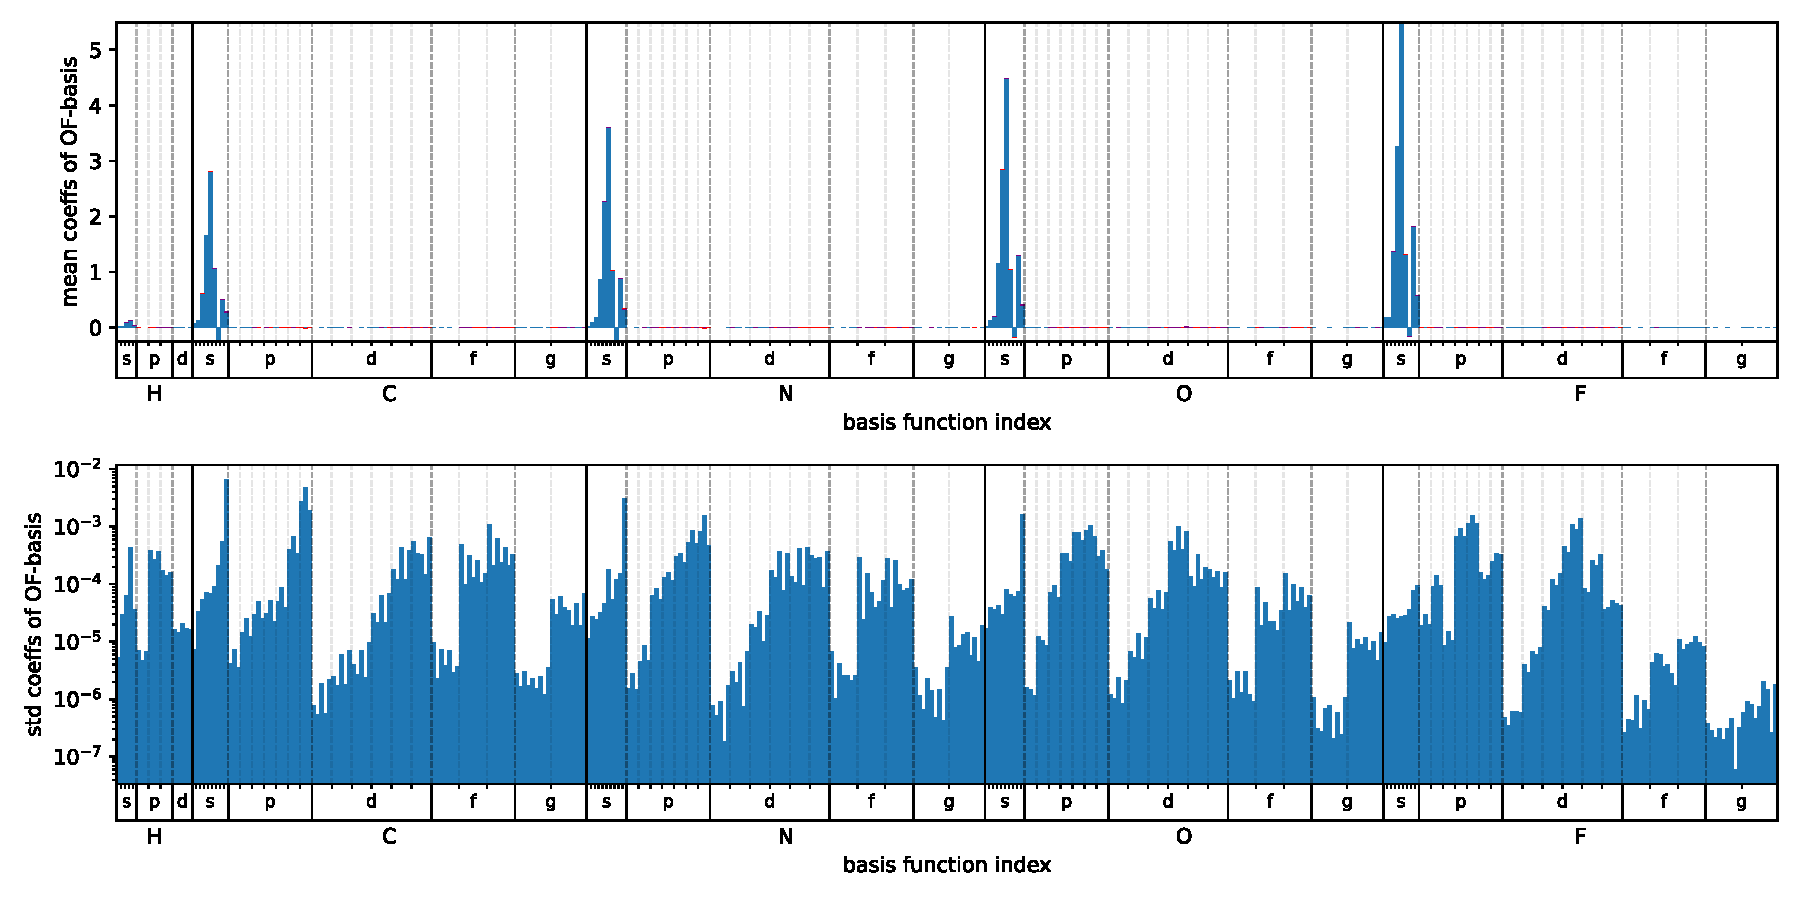
\includegraphics[width=0.9\textwidth]{chapters/results/results_images/var_coeffseven_tempered_3.0}
    \caption{The mean values(top) and the standart deviation(bottom) of the coefficients of an even tempered basis set with $\beta = 3.0$} \label{fig:var_coeffseven_tempered_3.0}
    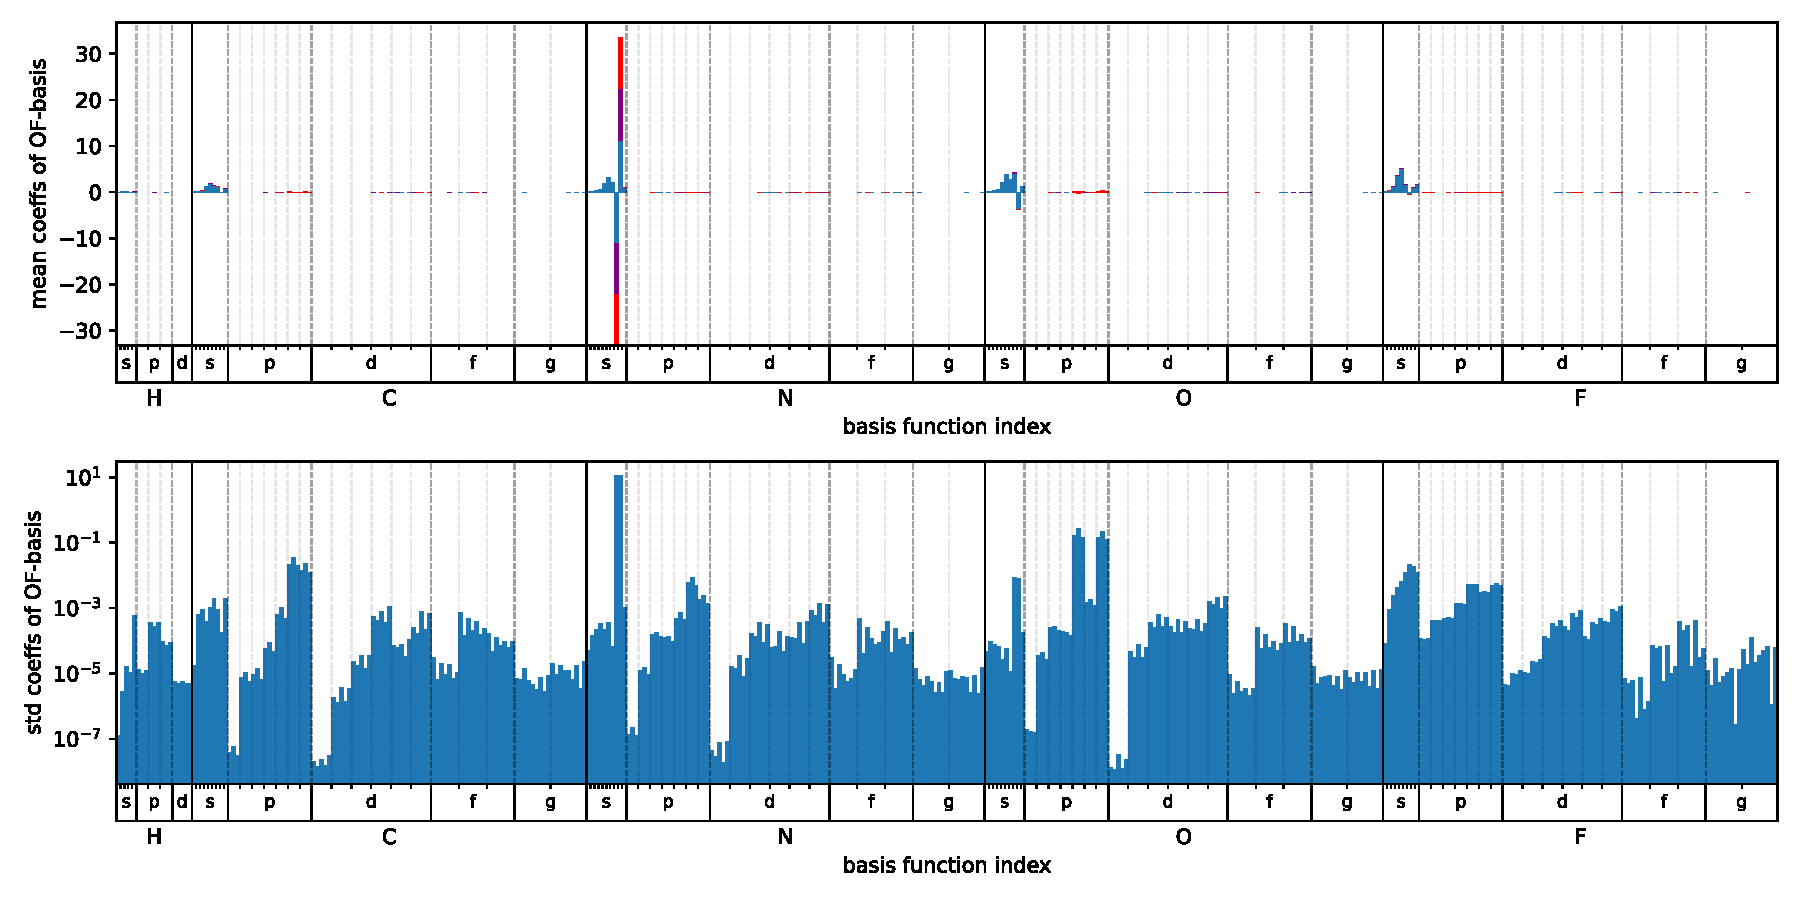
\includegraphics[width=0.9\textwidth]{chapters/results/results_images/var_coeffsfitted_basis_3.0}
        \caption{The mean values(top) and the standart deviation(bottom) of the coefficients of an basis set  fitted from even tempered with $\beta = 3.0$ without regularisation} \label{var_coeffsfitted_basis_3.0}
    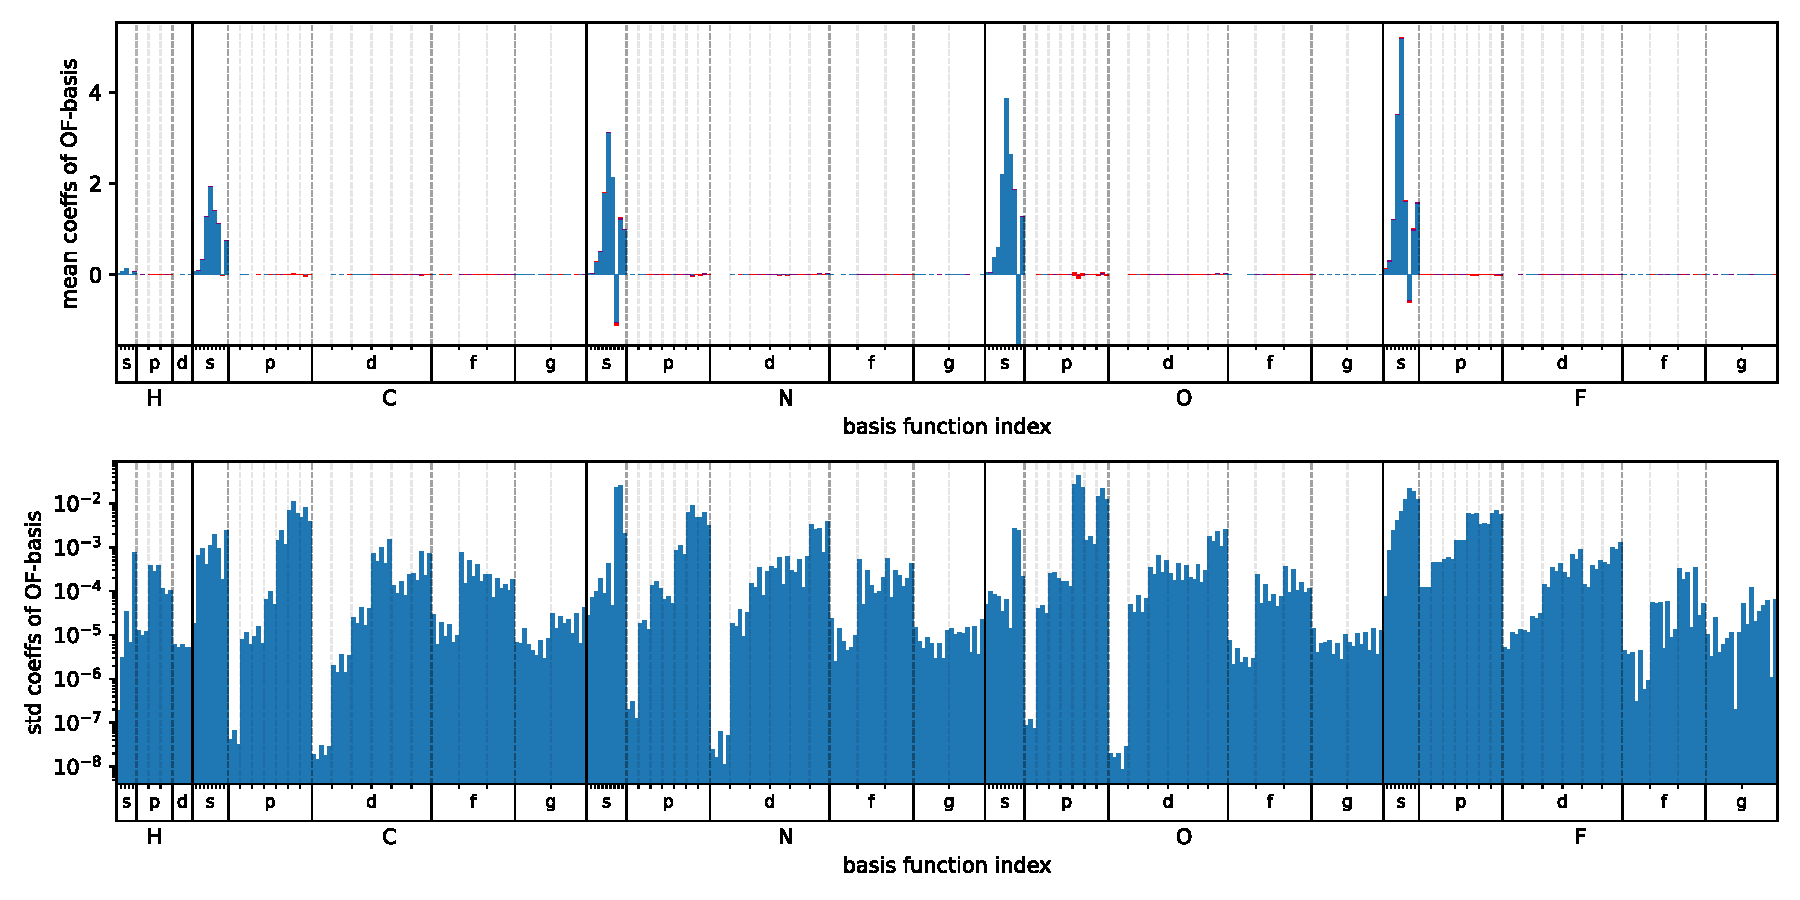
\includegraphics[width=0.9\textwidth]{chapters/results/results_images/var_coeffsfitted_regularized_basis_3.0}
        \caption{The mean values(top) and the standart deviation(bottom) of the coefficients of an basis set  fitted from even tempered with $\beta = 3.0$ after finetuning with regularisation} \label{var_coeffsfitted_regularized_basis_3.0}
\end{figure}

This can be seen when looking at an fitted basis set, initialized as even_tempered 3.0. We calculate the statistics of the coefficients of the individual basis functions for the first 1000 molecules of qm9
 Where the standart deviation is computed using A running STD implementation following welfords algorithm \cite{Welford}. 
 The following plots show how the metrics change after aplliing these additional sidelosses starting with the previously best performing basis sets.
 After applying these algorithms the standart deviation of the is much more evenly distributed over the coefficients. 
 Which also results in smoother training.
In figure\ref{fig:var_coeffseven_tempered_3.0} are the mean coeffihave moved very close together and lead to quite unstable coefficients.

\section{Comparison of the different fitted basis sets}
We are now going to compare different the performance of different basis sets.
\begin{table}
\centering
\tiny
\begin{tabular}{|l|ccc|ccccc|ccccc|ccccc|ccccc|}
\hline
& \multicolumn{3}{c|}{H} & \multicolumn{5}{c|}{C} & \multicolumn{5}{c|}{N} & \multicolumn{5}{c|}{O} & \multicolumn{5}{c|}{F} \\
Basis Set & s & p & d & s & p & d & f & g & s & p & d & f & g & s & p & d & f & g & s & p & d & f & g \\
\hline
even\_tempered\_1.5 & 12 & 7 & 2 & 25 & 17 & 15 & 7 & 4 & 25 & 18 & 15 & 7 & 4 & 25 & 18 & 16 & 7 & 4 & 25 & 18 & 16 & 7 & 4 \\
even\_tempered\_2.0 & 7 & 4 & 1 & 15 & 10 & 9 & 4 & 3 & 15 & 11 & 9 & 4 & 3 & 15 & 11 & 9 & 5 & 3 & 15 & 11 & 9 & 5 & 3 \\
even\_tempered\_2.5 & 6 & 3 & 1 & 11 & 8 & 7 & 3 & 2 & 11 & 8 & 7 & 4 & 2 & 11 & 8 & 7 & 4 & 2 & 11 & 8 & 7 & 4 & 2 \\
even\_tempered\_3.0 & 5 & 3 & 1 & 9 & 7 & 6 & 3 & 2 & 10 & 7 & 6 & 3 & 2 & 10 & 7 & 6 & 3 & 2 & 9 & 7 & 6 & 3 & 2 \\
def2-universal-jfit & 3 & 1 & 1 & 6 & 4 & 3 & 1 & 1 & 6 & 4 & 3 & 1 & 1 & 6 & 4 & 3 & 1 & 1 & 6 & 4 & 3 & 1 & 1 \\
fitted basis 2.5 & 6 & 3 & 1 & 11 & 8 & 7 & 3 & 2 & 11 & 8 & 7 & 4 & 2 & 11 & 8 & 7 & 4 & 2 & 11 & 8 & 7 & 4 & 2 \\
fitted reg. basis 2.5 & 6 & 3 & 1 & 11 & 8 & 7 & 3 & 2 & 11 & 8 & 7 & 4 & 2 & 11 & 8 & 7 & 4 & 2 & 11 & 8 & 7 & 4 & 2 \\
fitted basis 3.0 & 5 & 3 & 1 & 9 & 7 & 6 & 3 & 2 & 10 & 7 & 6 & 3 & 2 & 10 & 7 & 6 & 3 & 2 & 9 & 7 & 6 & 3 & 2 \\
fitted reg basis 3.0 & 5 & 3 & 1 & 9 & 7 & 6 & 3 & 2 & 10 & 7 & 6 & 3 & 2 & 10 & 7 & 6 & 3 & 2 & 9 & 7 & 6 & 3 & 2 \\
\hline
\end{tabular}
\caption{Detailed comparison of irreducible representations for different basis sets. For each atom, the number of basis functions is shown for each angular momentum (s, p, d, f, g). Hydrogen only includes s, p, and d functions. Each number represents the count of basis functions for that specific angular momentum. \footnote{Formatting done by claude}}
\label{tab:basis-comparison-detailed}
\end{table}

We are going to compare the different fitted basis sets using the same metrics as before for the different density fitting methods in section \ref{metrics}.


 At last we are going to compare the performance of a typical transformer model trained on the different fitted basis sets when doing denop and find out that while they aren't better at fitting the produced labels, they still perform better when compared to the orbital free density and lower the theoretical best performance.

\begin{figure}
    \centering
    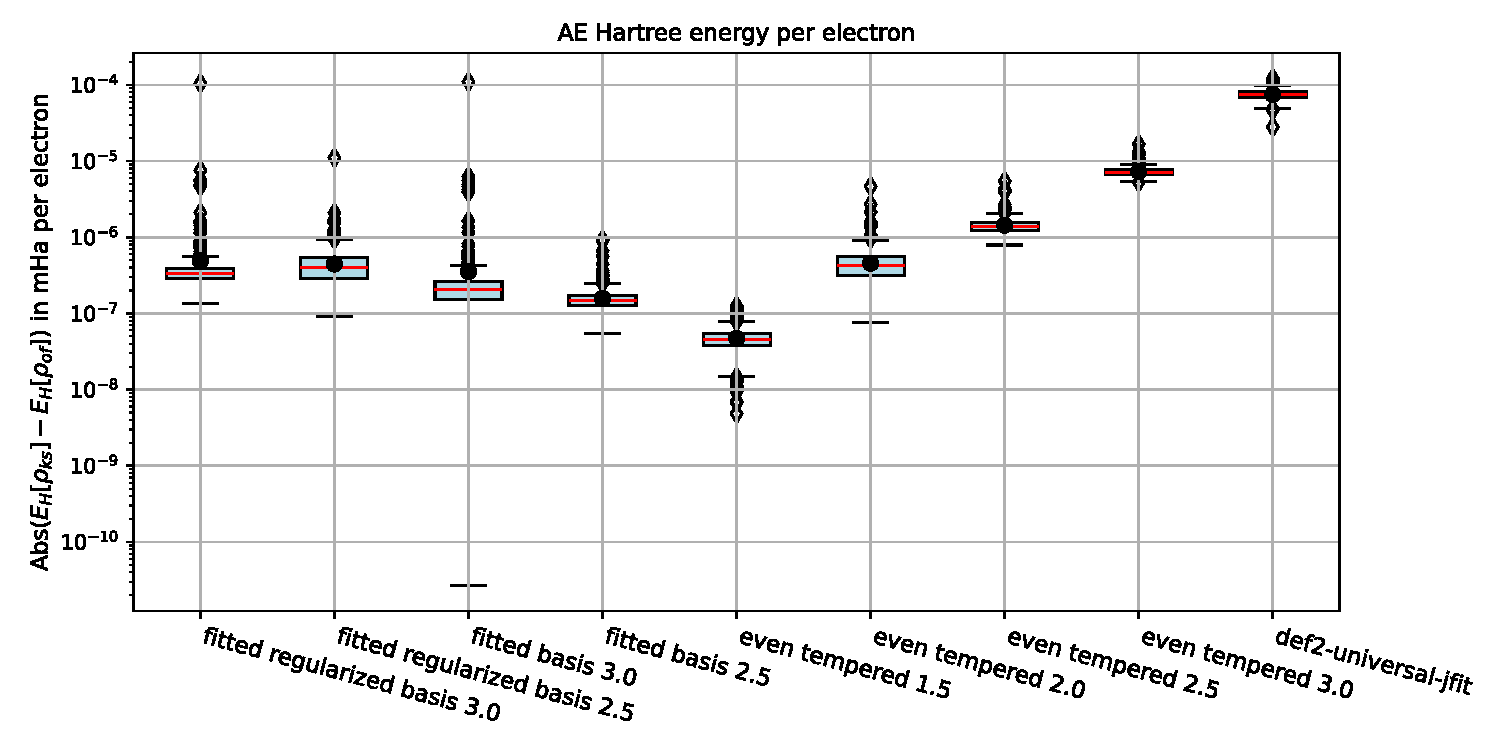
\includegraphics[width=0.9\textwidth]{chapters/results/results_images/AE_hartree_energy_on_hartree+external_MOFDFT_for_different_basis_sets}
    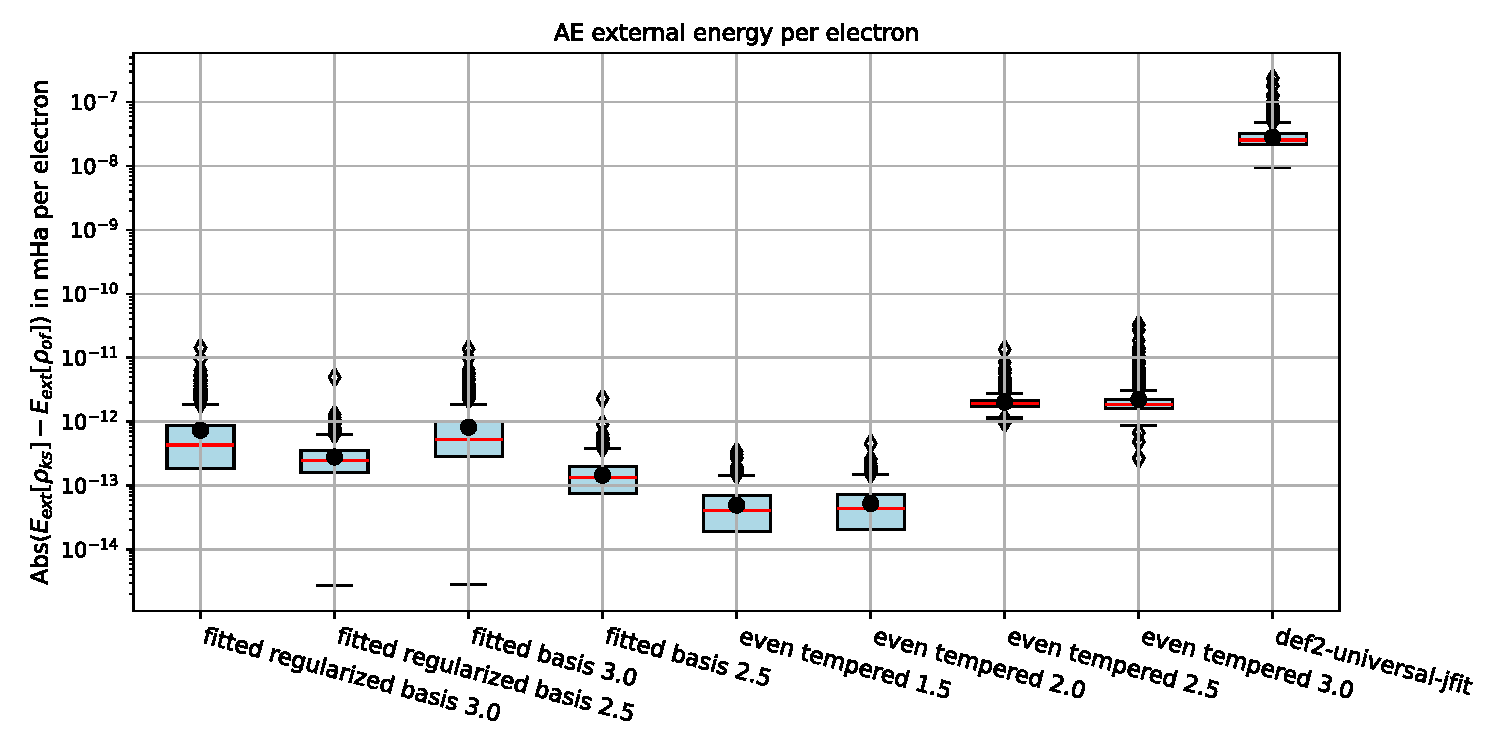
\includegraphics[width=0.9\textwidth]{chapters/results/results_images/AE_ext_energy_on_hartree+external_MOFDFT_for_different_basis_sets}
    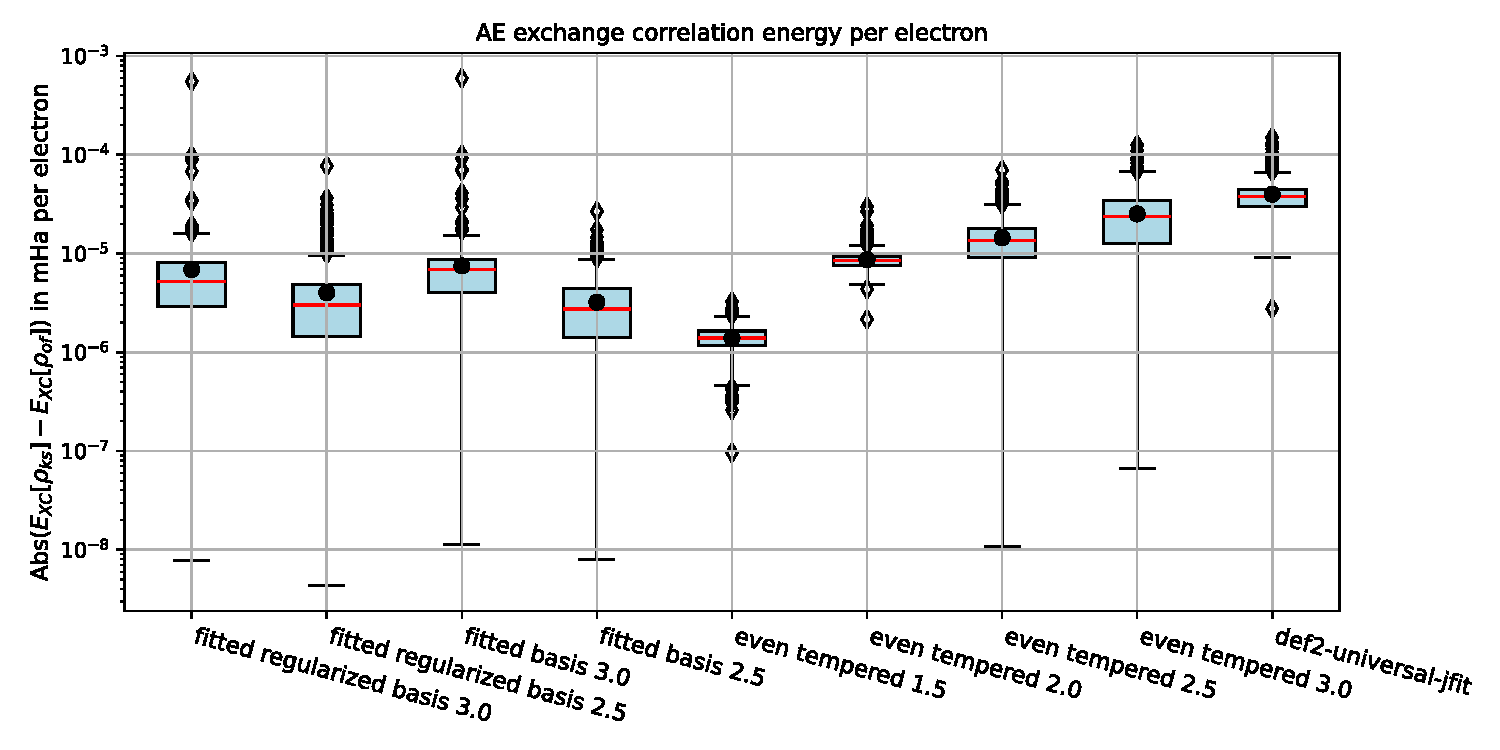
\includegraphics[width=0.9\textwidth]{chapters/results/results_images/AE_xc_energy_on_hartree+external_MOFDFT_for_different_basis_sets}
    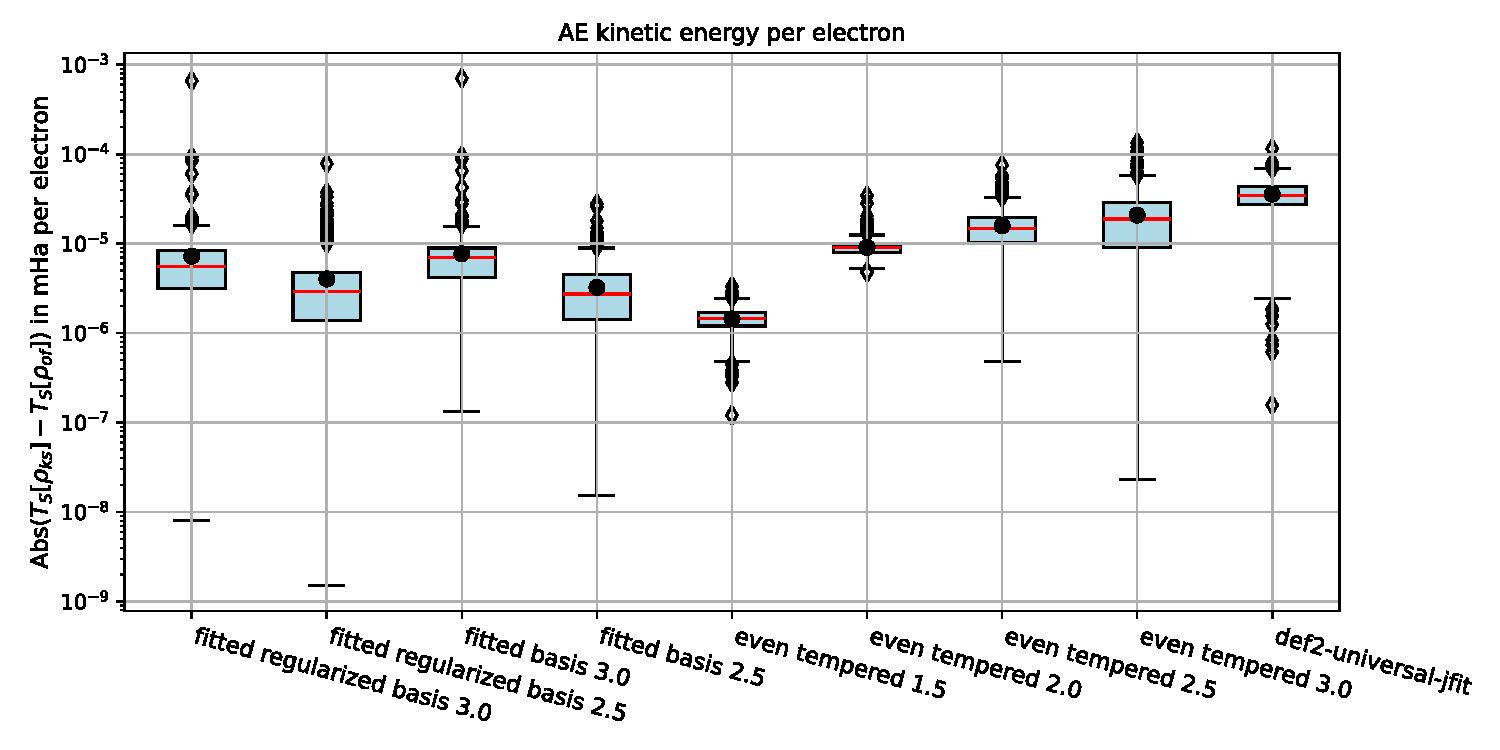
\includegraphics[width=0.9\textwidth]{chapters/results/results_images/AE_kin_energy_on_hartree+external_MOFDFT_for_different_basis_sets}
    \caption{Boxplots(\ref{boxplots}) of the AE for the different energies on the fitted basis sets}
\end{figure}
\begin{figure}
    \centering
        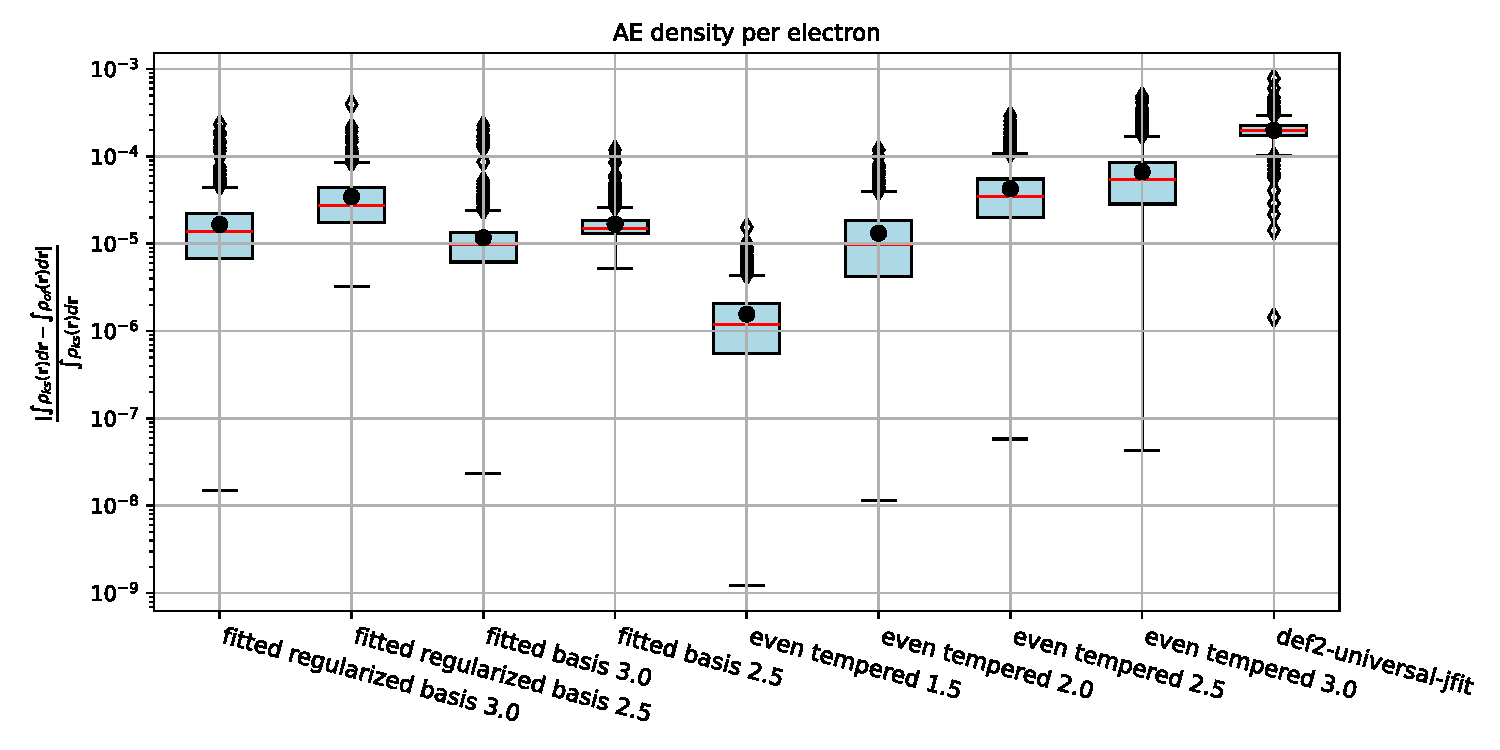
\includegraphics[width=0.9\textwidth]{chapters/results/results_images/AE_density_on_hartree+external_MOFDFT_for_different_basis_sets}
    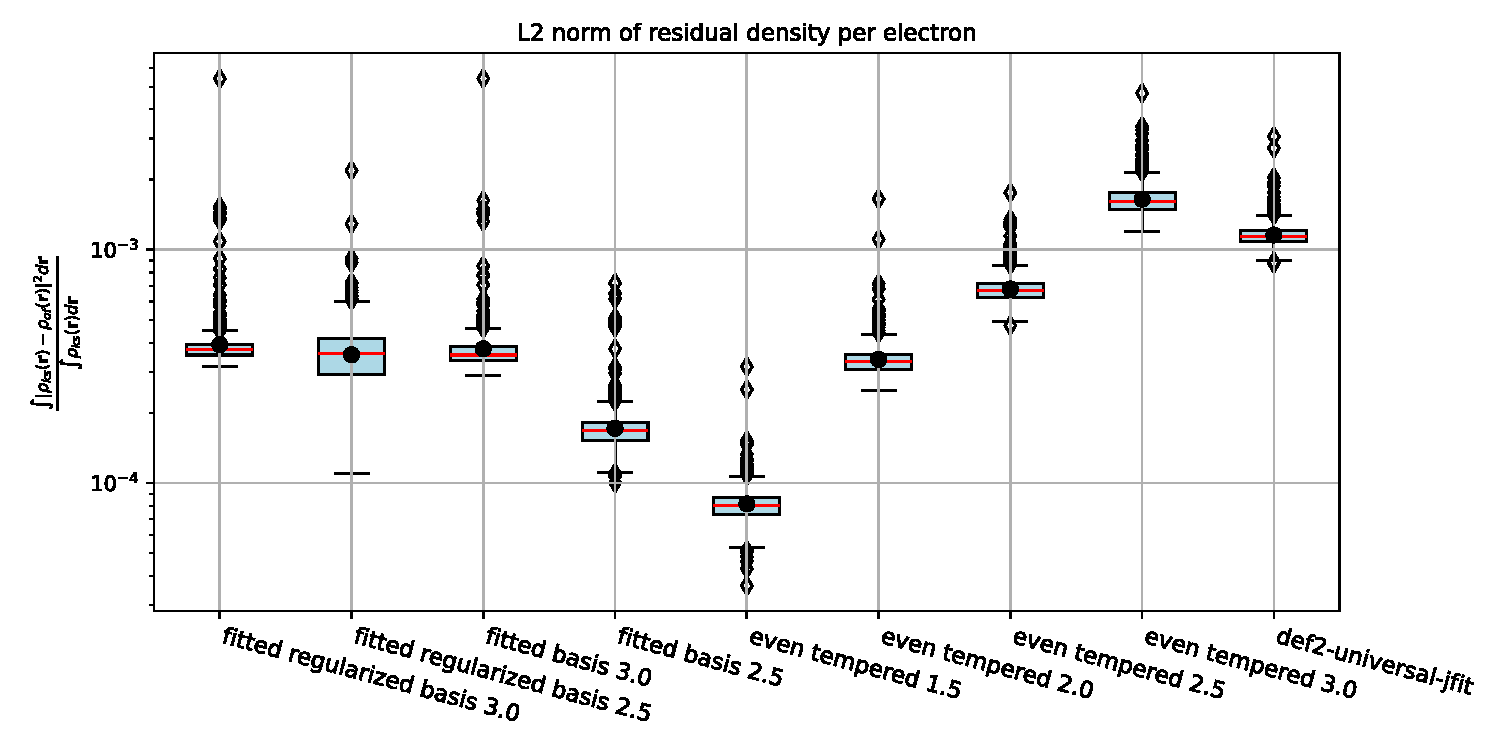
\includegraphics[width=0.9\textwidth]{chapters/results/results_images/L2_residual_densities_on_hartree+external_MOFDFT_for_different_basis_sets}
    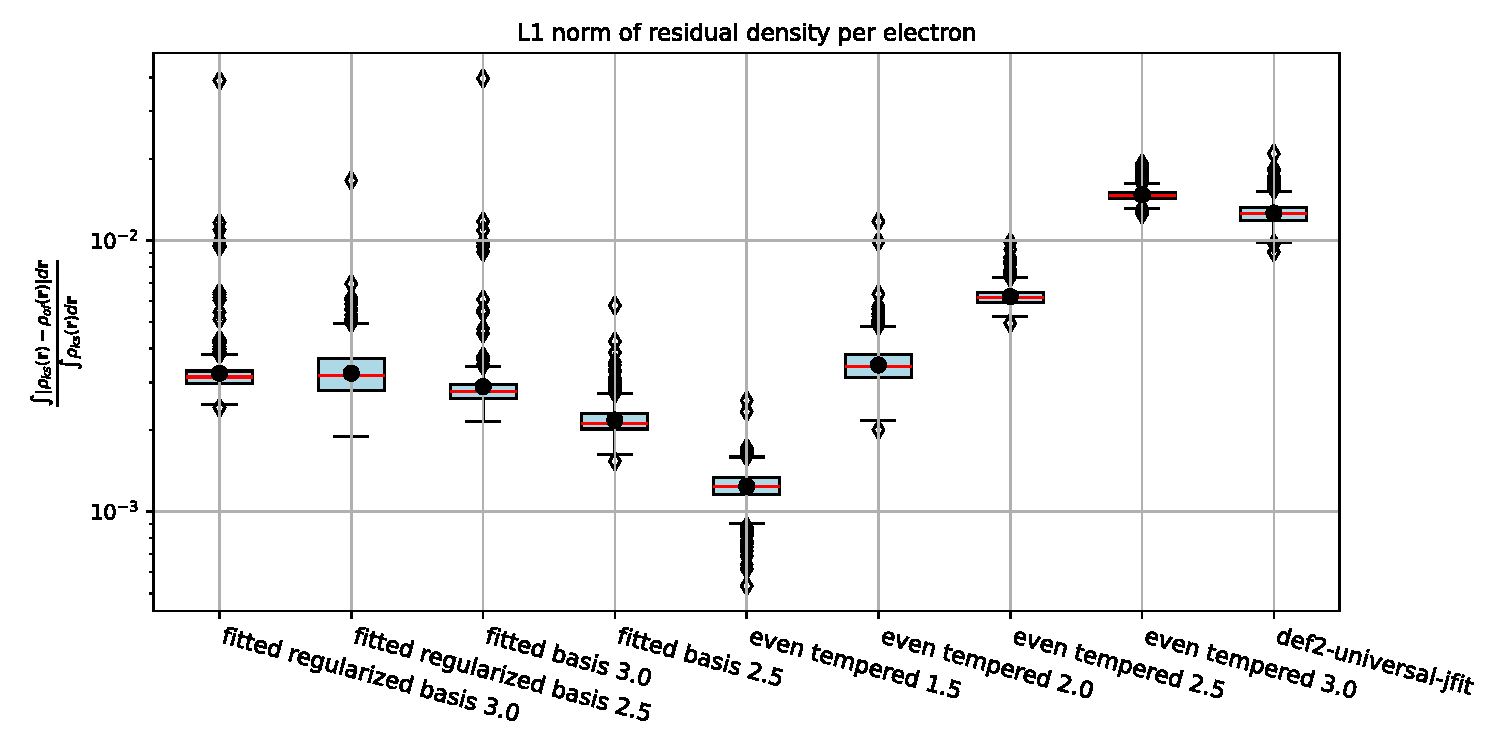
\includegraphics[width=0.9\textwidth]{chapters/results/results_images/L1_residual_densities_on_hartree+external_MOFDFT_for_different_basis_sets}
    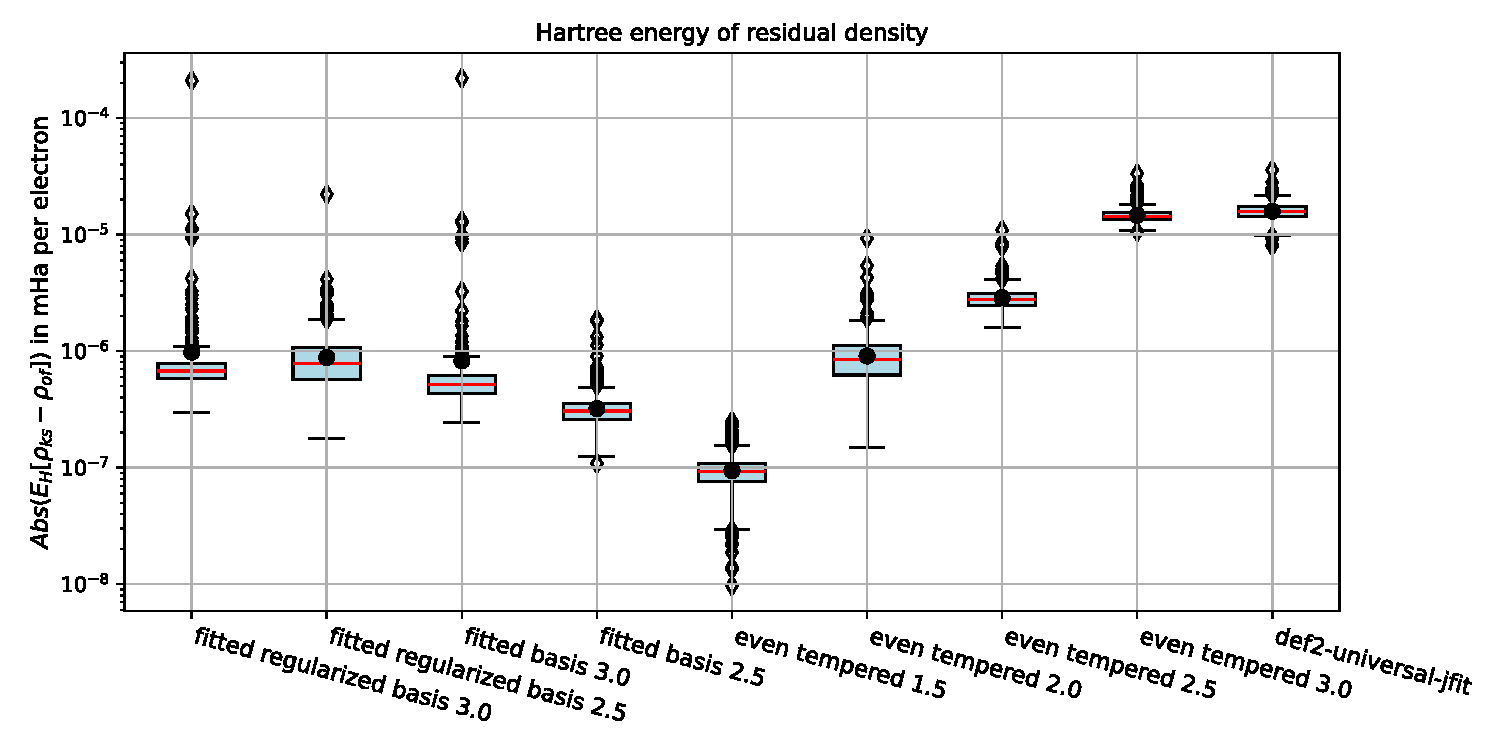
\includegraphics[width=0.9\textwidth]{chapters/results/results_images/L2_residual_hartree_on_hartree+external_MOFDFT_for_different_basis_sets}
\caption{Boxplots(\ref{boxplots}) to compare the overall dfit of the denisty of the fitted basis sets to the target density}
\end{figure}
    \begin{figure}
    \centering
    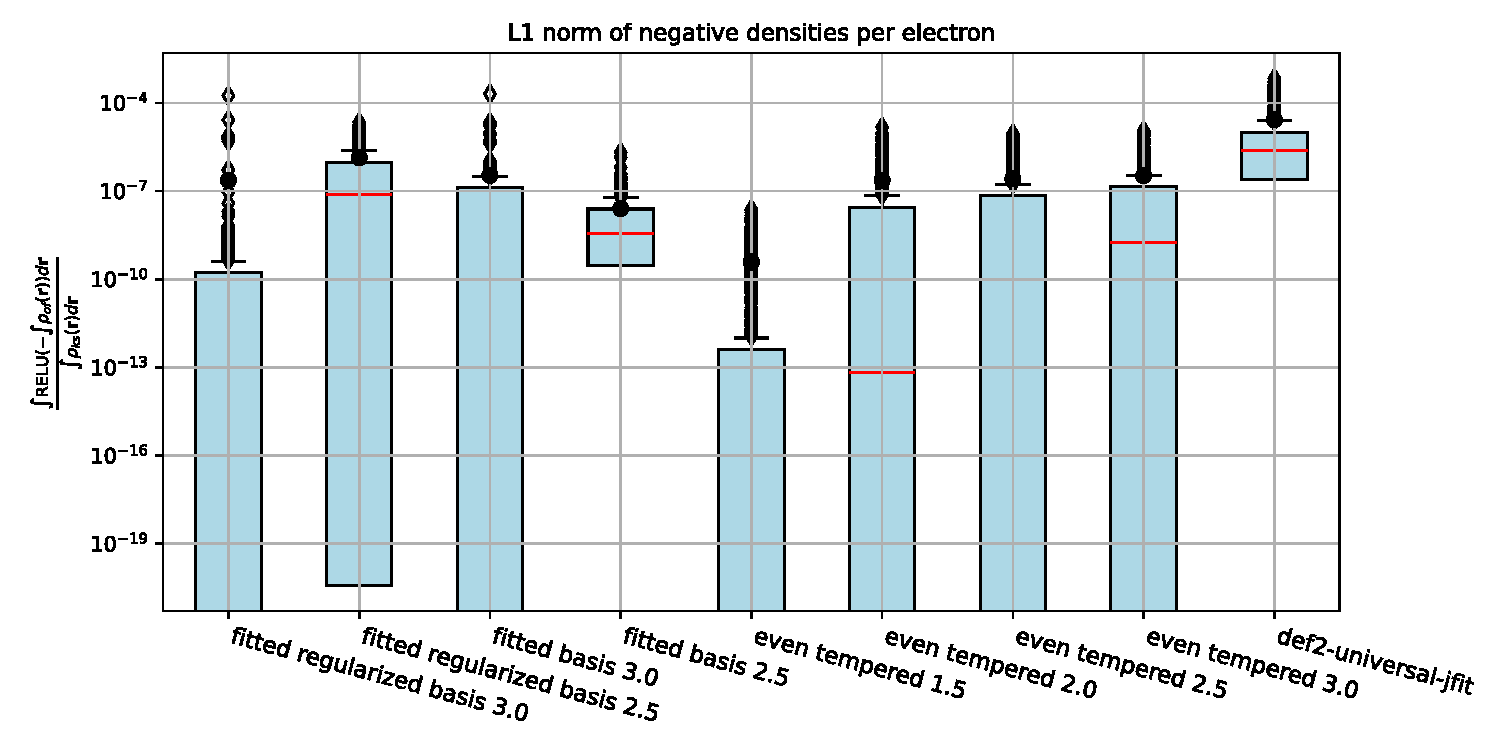
\includegraphics[width=0.9\textwidth]{chapters/results/results_images/L1_negative_densities_on_hartree+external_MOFDFT_for_different_basis_sets}
    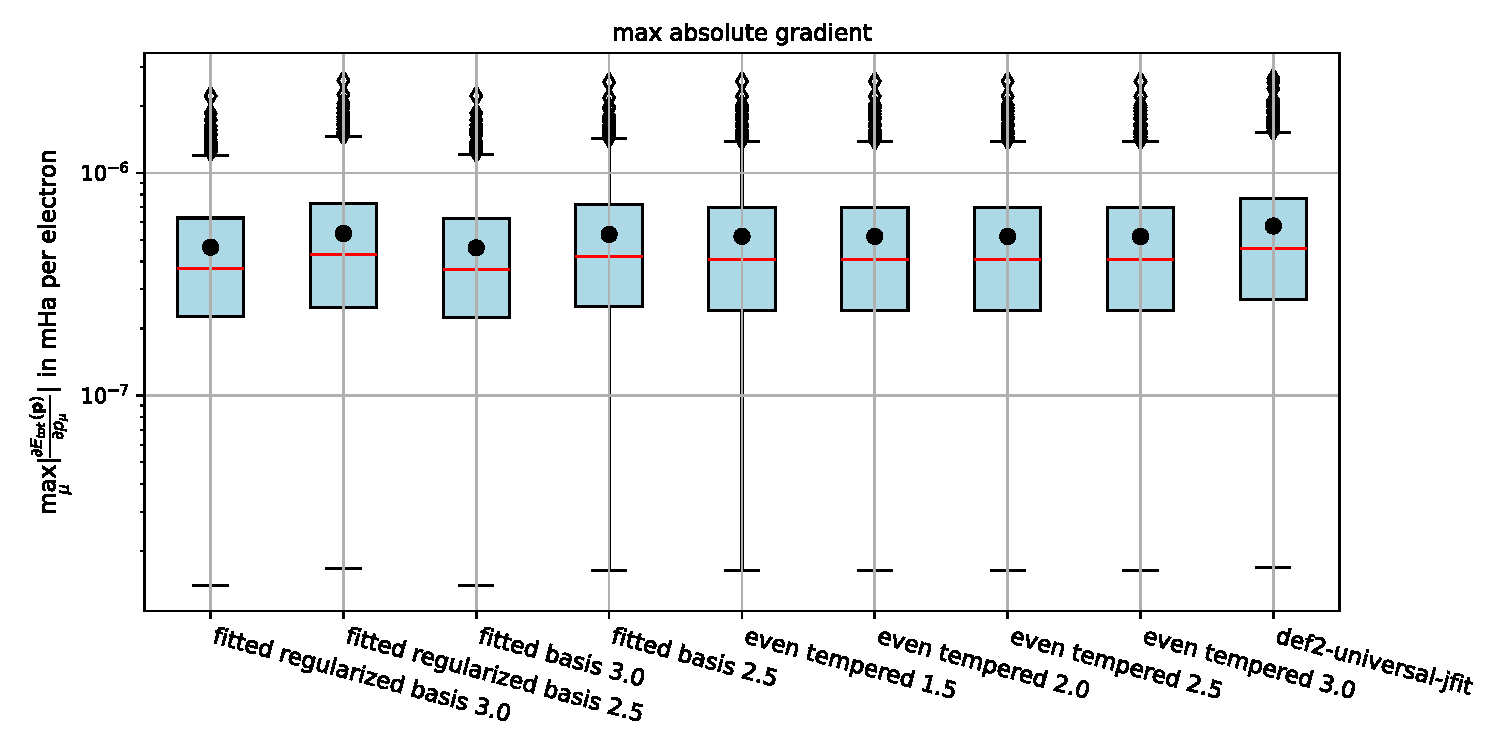
\includegraphics[width=0.9\textwidth]{chapters/results/results_images/max_abs_gradient_on_hartree+external_MOFDFT_for_different_basis_sets}
    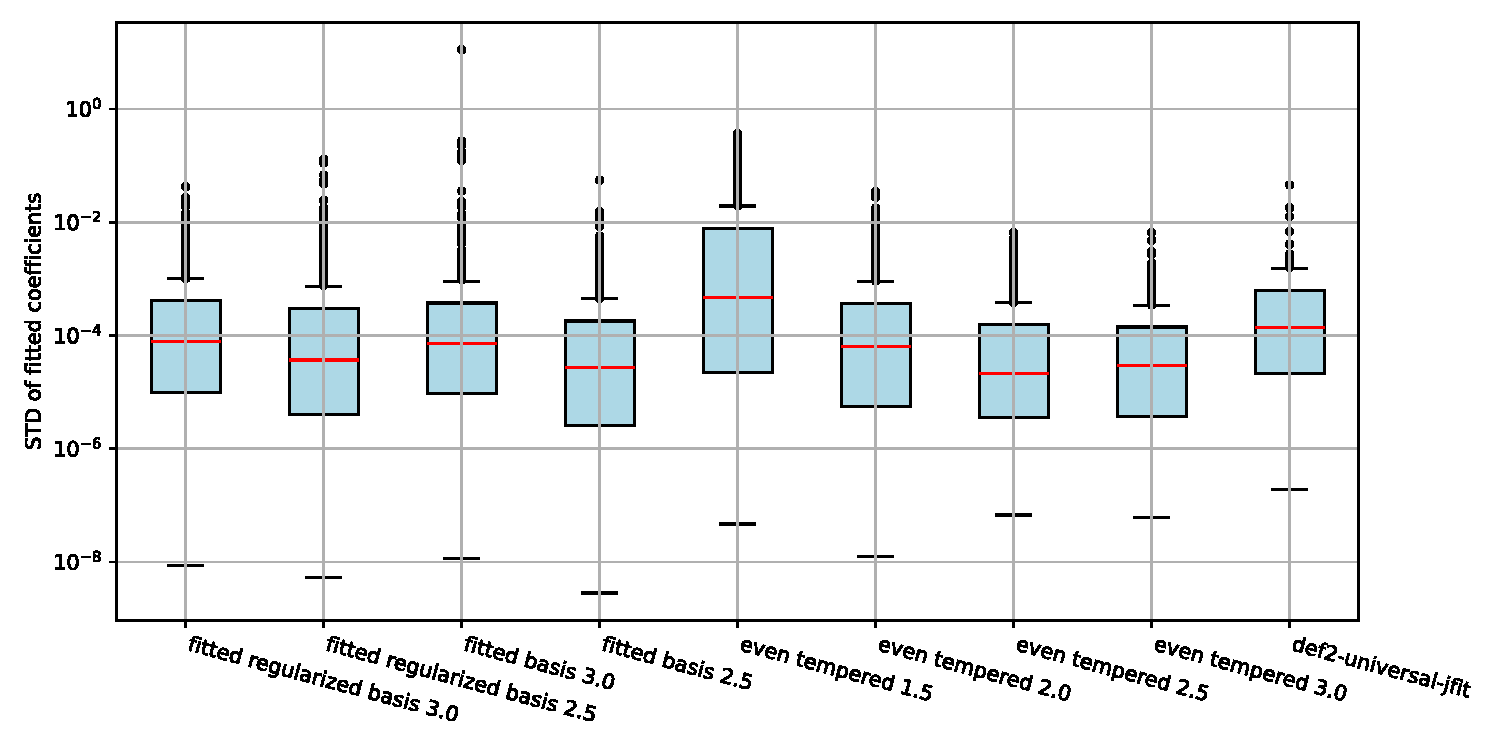
\includegraphics[width=0.9\textwidth]{chapters/results/results_images/var_basis_sets}
    \caption{Boxplots(\ref{boxplots}) analysing the different additional metrics for the fitted basis sets}
\end{figure}


 \begin{figure}
   \centering
   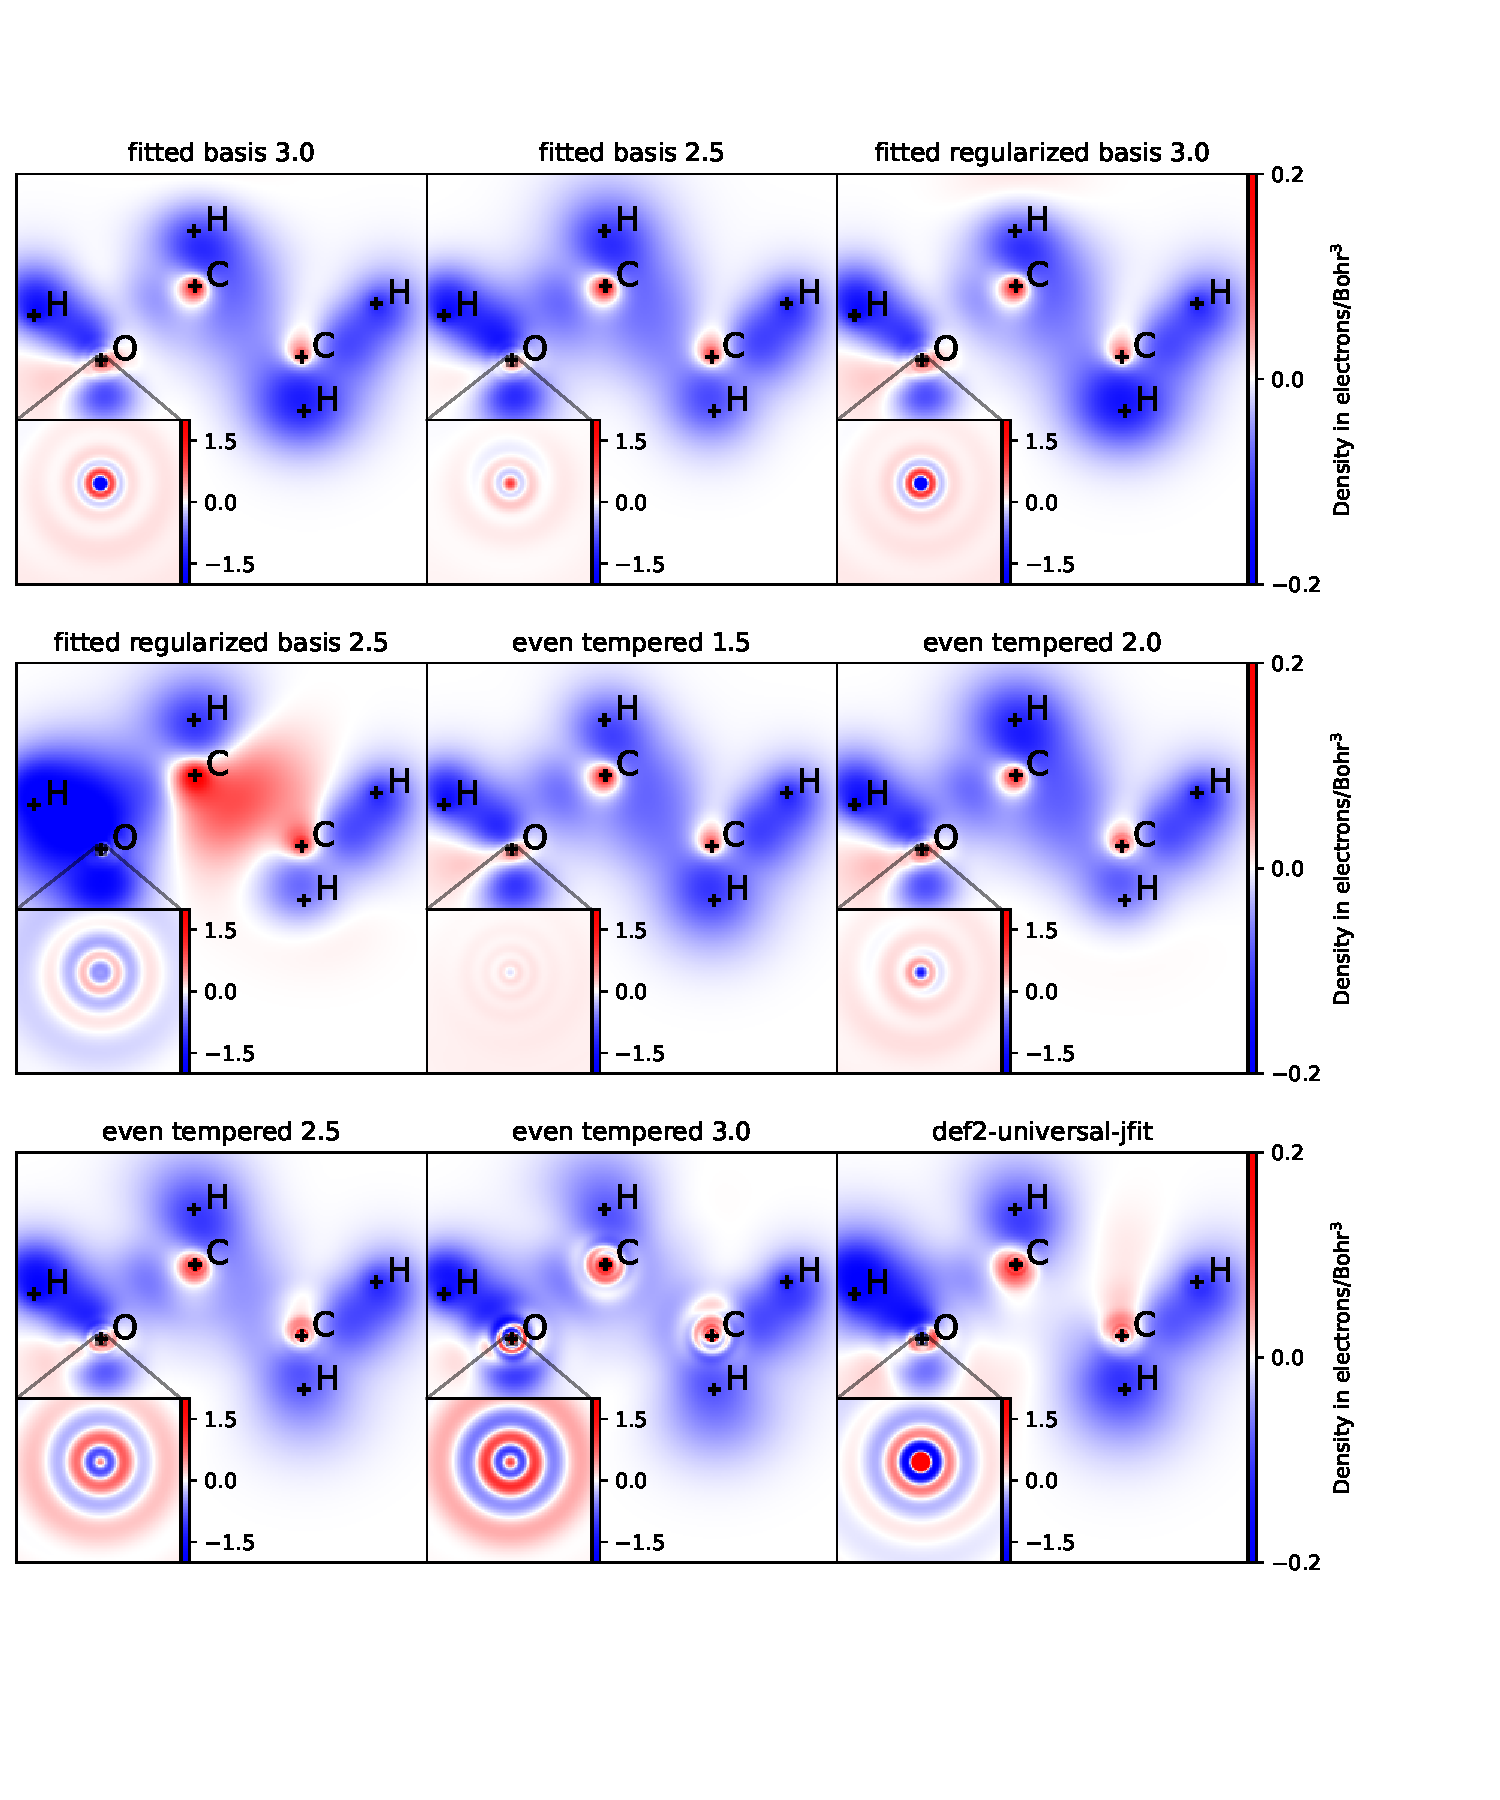
\includegraphics[width=1\textwidth]{chapters/results/results_images/basis_set_slices.pdf}
     \caption{Slices of the fitted density with density fitting method hartree+external Mofdft using different basis sets}
 \end{figure}



\begin{figure}
   \centering
   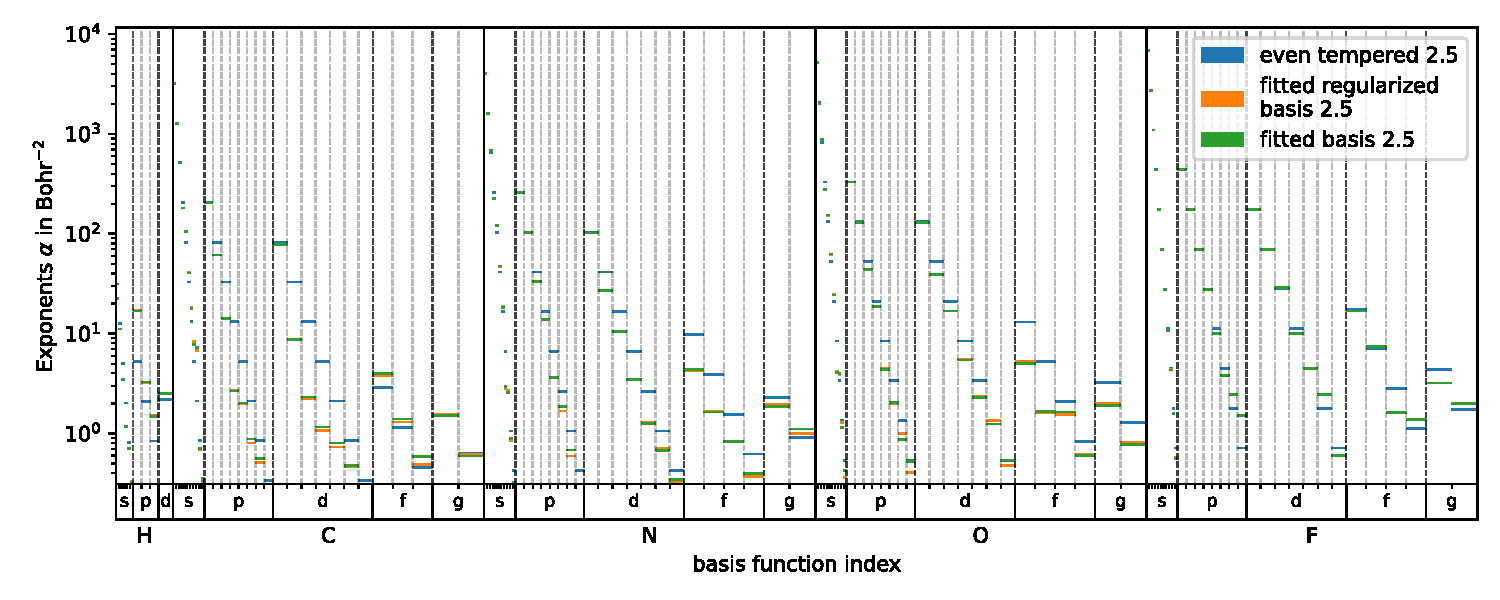
\includegraphics[width=0.6\textwidth]{chapters/results/results_images/basis_functions_with_size2.5}
   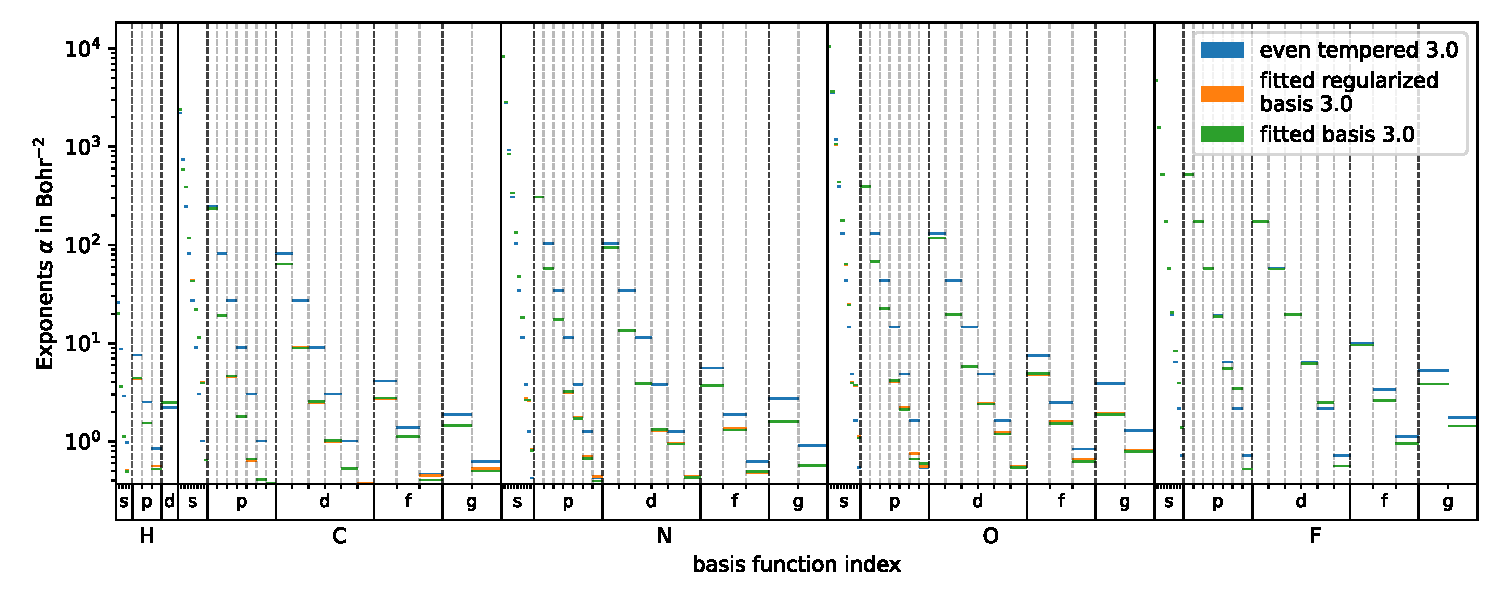
\includegraphics[width=0.6\textwidth]{chapters/results/results_images/basis_functions_with_size3.0}
    \caption{}
\end{figure}








